With Test-Driven Development (TDD), before writing the actual code, the developer writes unit test cases for the new functionality they are about to implement~\cite{beckTestDriven}. The method is related to the test-first practise used in eXtreme Programming (XP)~\cite{beckXP} but today it’s also used on it’s on together with other development methods~\cite{MSNET}. TDD was used in the 1960’ in the NASA Project Mercury~\cite{NASA} and then rediscovered by Kent Beck (who created XP) in 2003 who claims that it encourages simple design and inspires confidence~\cite{beckXP}. In XP the developers break down things to be implemented into smaller problems, also known as stories. When using TDD with XP, the workflow is according to the scheme below(INSERT BILD REF). After a few test cases are developed the code to make them pass are implemented. Generally the test cases wont even compile before the code is implemented. If the test cases pass, the developer either writes more test cases for the next piece of functionality or moves on to the next story depending on whether the previous story is finished or not. If the test cases fail the developer has to go back and rework the newly implemented code.

\begin{figure*}
\begin{center}
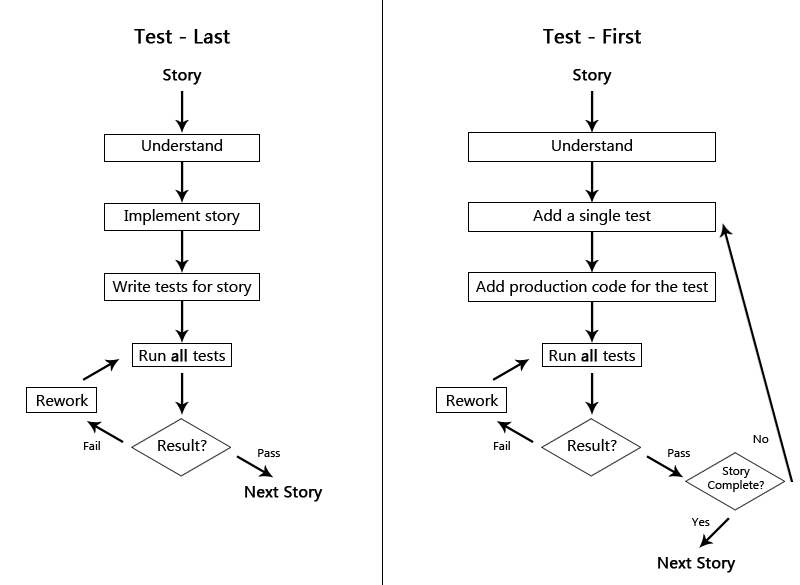
\includegraphics[scale=0.60]{tdd.png}
\caption{Shows the diffrence between the Test-Last and Test-First workflow}
\end{center}
\end{figure*}


By focusing on writing only code necessary to pass tests, designs can be cleaner and clearer than is often achieved by other methods~\cite{beckXP}. When used in XP projects TDD help with the method practice “Simple Design” which basically is keeping the code as simple as possible and only implement functionality that is needed. By doing this the code is easier to work with and it simplifies future integrations. 


When performing TDD developers usually use some sort of test tool. An example of this is JUnit which can be used when developing in Java. JUnit includes a set of assert statements which can be used to verify the output given when unit testing. It also provides Before- and After statements which helps the developer to set up and tear down variables that are needed for several tests. With this functionality, test tools helps the developer manage the vast amount of test cases that are produced.


There are several statements that TDD increasing code quality and productivity~\cite{beckXP}~\cite{erdogmus}. For instance they argue that the test cases are more efficient since the tests have been developed from requirements instead of existing code. However there are others who showed studies that there’s no difference or even a decrease in the overall results~\cite{tddInvest}~\cite{mullerandhagner}. In Section 4 we will try to determine which is more likely based on studies and articles.